\documentclass[11pt]{article} 
\usepackage[english]{babel}
\usepackage[utf8]{inputenc}
\usepackage[margin=0.5in]{geometry}
\usepackage{amsmath}
\usepackage{amsthm}
\usepackage{amsfonts}
\usepackage{amssymb}
\usepackage[usenames,dvipsnames]{xcolor}
\usepackage{graphicx}
\usepackage[siunitx]{circuitikz}
\usepackage{tikz}
\usepackage[colorinlistoftodos, color=orange!50]{todonotes}
\usepackage{hyperref}
\usepackage[numbers, square]{natbib}
\usepackage{fancybox}
\usepackage{epsfig}
\usepackage{soul}
\usepackage[framemethod=tikz]{mdframed}
\usetikzlibrary{positioning, automata, backgrounds}
\usepackage[shortlabels]{enumitem}
\usepackage[version=4]{mhchem}
\usepackage{multicol}
\usepackage{forest}
\usepackage{mathtools}
\usepackage{comment}
\usepackage{enumitem}
\usepackage[utf8]{inputenc}
\usepackage[linesnumbered,ruled,vlined]{algorithm2e}
\usepackage{listings}
\usepackage{color}
\usepackage[numbers]{natbib}
\usepackage{subfiles}
\usepackage{tkz-berge}
\usepackage{pythonhighlight}


\newtheorem{prop}{Proposition}[section]
\newtheorem{thm}{Theorem}[section]
\newtheorem{lemma}{Lemma}[section]
\newtheorem{cor}{Corollary}[prop]

\theoremstyle{definition}
\newtheorem{definition}{Definition}

\theoremstyle{definition}
\newtheorem{required}{Problem}

\theoremstyle{definition}
\newtheorem{ex}{Example}

\newcommand{\interval}[4]{\draw (#2, #1) -- (#3, #1); % Usage: \interval{height}{start}{end}{label}
\draw (#2, #1-0.11) -- (#2, #1+0.11); % draw left whisker
\draw (#3, #1-0.11) -- (#3, #1+0.11); % draw right whisker
\node[] at (#2-0.25, #1) {#4};
}

\setlength{\marginparwidth}{3.4cm}
%#########################################################

%To use symbols for footnotes
\renewcommand*{\thefootnote}{\fnsymbol{footnote}}
%To change footnotes back to numbers uncomment the following line
%\renewcommand*{\thefootnote}{\arabic{footnote}}

% Enable this command to adjust line spacing for inline math equations.
% \everymath{\displaystyle}

% _______ _____ _______ _      ______ 
%|__   __|_   _|__   __| |    |  ____|
%   | |    | |    | |  | |    | |__   
%   | |    | |    | |  | |    |  __|  
%   | |   _| |_   | |  | |____| |____ 
%   |_|  |_____|  |_|  |______|______|
%%%%%%%%%%%%%%%%%%%%%%%%%%%%%%%%%%%%%%%

\title{
\normalfont \normalsize 
\textsc{CSCI 3104 Spring 2022 \\ 
Instructors: Profs. Chen and Layer} \\
[10pt] 
\rule{\linewidth}{0.5pt} \\[6pt] 
\huge Problem Set 2 \\
\rule{\linewidth}{2pt}  \\[10pt]
}
%\author{}
\date{}

\begin{document}

\definecolor {processblue}{cmyk}{0.96,0,0,0}
\definecolor{processred}{rgb}{200, 0, 0}
\definecolor{processgreen}{rgb}{0, 255, 0}
\DeclareGraphicsExtensions{.png}
\DeclareGraphicsExtensions{.gif}
\DeclareGraphicsExtensions{.jpg}

\maketitle


%%%%%%%%%%%%%%%%%%%%%%%%%
%%%%%%%%%%%%%%%%%%%%%%%%%%
%%%%%%%%%%FILL IN YOUR NAME%%%%%%%
%%%%%%%%%%AND STUDENT ID%%%%%%%%
%%%%%%%%%%%%%%%%%%%%%%%%%%
\noindent
Due Date \dotfill February 1, 2022 \\
Name \dotfill \textbf{Julia Troni} \\
Student ID \dotfill \textbf{109280095} \\
Collaborators \dotfill \textbf{Me, myself and I}

\tableofcontents

\section{Instructions}
 \begin{itemize}
	\item The solutions \textbf{should be typed}, using proper mathematical notation. We cannot accept hand-written solutions. \href{http://ece.uprm.edu/~caceros/latex/introduction.pdf}{Here's a short intro to \LaTeX.}
	\item You should submit your work through the \textbf{class Canvas page} only. Please submit one PDF file, compiled using this \LaTeX \ template.
	\item You may not need a full page for your solutions; pagebreaks are there to help Gradescope automatically find where each problem is. Even if you do not attempt every problem, please submit this document with no fewer pages than the blank template (or Gradescope has issues with it).

	\item You are welcome and encouraged to collaborate with your classmates, as well as consult outside resources. You must \textbf{cite your sources in this document.} \textbf{Copying from any source is an Honor Code violation. Furthermore, all submissions must be in your own words and reflect your understanding of the material.} If there is any confusion about this policy, it is your responsibility to clarify before the due date. 

	\item Posting to \textbf{any} service including, but not limited to Chegg, Reddit, StackExchange, etc., for help on an assignment is a violation of the Honor Code.

	\item You \textbf{must} virtually sign the Honor Code (see Section \ref{HonorCode}). Failure to do so will result in your assignment not being graded.
\end{itemize}


\section{Honor Code (Make Sure to Virtually Sign)} \label{HonorCode}

\begin{required}
\begin{itemize}
\item My submission is in my own words and reflects my understanding of the material.
\item Any collaborations and external sources have been clearly cited in this document.
\item I have not posted to external services including, but not limited to Chegg, Reddit, StackExchange, etc.
\item I have neither copied nor provided others solutions they can copy.
\end{itemize}

%\noindent In the specified region below, clearly indicate that you have upheld the Honor Code. Then type your name. 
\end{required}

\begin{proof}[I agree to the above, Julia Troni.]
%% Typing "I agree to the above," followed by your name is sufficient.
\end{proof}


%%%%%%%%%%%%%%%%%%%%%%%%%%%%%%%%%%%%%%%%%%%%%%%%%%
\newpage
\section{Standard 5- BFS and DFS}
\subsection{Problem \ref{DFS1}}
\begin{required} \label{DFS1}
Consider a \textsf{Modified Connectivity} problem:
\begin{itemize}
\item \textsf{Instance:} Let $G(V, E)$ be a simple, undirected graph. Let $s, t \in V(G)$.
\item \textsf{Decision:} Given an integer $k\geq 1$,  is there a shortest path from $s$ to $t$ in $G$ that consists of $k$ edges? Here the length/weight of a path is defined as the number of edges of the path. 
\end{itemize}

\noindent \\ Do the following. [\textbf{Note:} There are parts (a) and (b). Part (b) is on the next page.]
\begin{enumerate}[label=(\alph*)]
\item Design an algorithm to solve the $\textsf{Modified Connectivity}$ problem. Your solution should provide enough detail that a CSCI 2270 student could reasonably be expected to implement your solution.
\begin{proof}[Answer for Part (a)]
%Your answer goes here

The following pseudo code shows an algorithm to solve the Modified Connectivity Problem. The function $ModifiedConnectivity$ uses a modified BFS algorithm to find the shortest path and check if it is equal to $k$. It takes input of the graph $G$, the starting vertex $s$, the vertex we wish to traverse to $t$, and $k$, the number of edges of the path. It will return true the path is equal to $k$, otherwise it will return false. 
\begin{itemize}
\item Begin by initializing 3 arrays a state array to hold if a vertex has been visited, a predecessor array that will track the parent node along the path, and a distance array to save how many edges it took to reach that vertex. Set all vertices to NEW (unvisited), all predecessors to NULL, and all distances to infinity  
\item Then set the distance of the start vertex, $s$, to 0. 
\item Make a FIFO queue with the start vertex and that predecessor, which is NULL. 
\item Then while the queue is not empty, dequeue a vertex, if it is marked as NEW, set it to OLD, save the predecessor, and increment the distance by $1$. Then for each neighbor of that vertex, add it to the queue. In this way we are traversing all the connected elements of graph, and due to the FIFO queue, we are traversing layer by layer and hence finding the shortest path. 
\item Once the while loop completes, check if the goal vertex, $t$, has been marked OLD and if that the distance is equal to $k$. If so, return true. Otherwise, return false.  \\
\end{itemize}
\begin{python}

#G is a simple undirected graph
#s is the starting vertex in G
#t is the vertex that we wish to traverse to
#k is the length of the path from s to t
#ModifiedConnectivity will return true if there is a shortest path from vertex s to t with k edges
def ModifiedConnectivity(Graph G, Vertex s, Vertex t, Integer k) {
	for i to n {
		state[i] = NEW 	#mark all vertices as unvisited
		pred[i] = NULL		#initialize array to hold predecessors 
		dist[i] = infinity 	#set all distances to infinity
	}

	dist[s] = 0 	#distance of s set to 0
	Q= newQueue(NULL, s) 	  #make a queue, with pred[s] and s. Very important that queue is FIFO 

	while Q is not empty {
		(p,x)= deQueue(Q) 	#get vertex x out of Q
		if state[x]==NEW {
			state[x]=OLD 	#mark it as visited
			pred[x]=p 	#save how we got to x
			dist[x]=dist[p]+1	 	#store the distance to x 
			for each neighbor y of x {
				enqueue(Q, (x,y)) 	#add y to the Q
			}
		}
	}

	if (state[t] == OLD && dist[t] ==k) { 	#if t has been visited and the distance to t is the same as k, then there does exist a path from s to t in G that consists of k edges
		return true
	}
	else {
		return false
	}
}
\end{python}
\end{proof}



\newpage
\item We say that the graph $G$ is \textit{connected} if for every pair of vertices $s, t \in V(G)$, there exists a path from $s$ to $t$. Design an algorithm to determine whether $G$ is connected. Your algorithm should only traverse the graph once - this means that you should \textbf{not} apply BFS or DFS more than once. Your solution should provide enough detail that a CSCI 2270 student could reasonably be expected to implement your solution.

\begin{proof}[Answer for Part (b)]
%Your answer goes here

The following pseudo code shows an algorithm to determine if $G$ is connected. The function $CheckConnected$ takes input of the graph $G$, the starting vertex, and the total number of nodes in the graph and it will return true if the graph is connected, otherwise it will return false. 
\begin{itemize}
\item Begin by initializing a count variable to 0. Then initialize a state array where the state of all the vertices in the graph is NEW, meaning unvisited.
\item Make a queue containing the start vertex, the queue can be FIFO or LIFO because either BFS or DFS will traverse all connected elements. 
\item Then while the queue is not empty, dequeue a vertex. If it marked NEW,  set it to OLD and increment the count variable by 1 and for each neighbor of that vertex, add it to the queue. In this way we are traversing all the elements of graph that are connected to the start vertex. 
\item Once the while loop completes, check if the count is equal to the number of nodes. If so, it indicates that we were able to reach every vertex from the starting vertex and thus the graph is connect so return true. If not, return false. \\
\end{itemize}

\begin{python}

#G is a graph that may or may not be connected
#s is the starting vertex in G
#NumNodes is the total number of nodes in a graph
#CheckConnected will return true if the graph is connected, otherwise it will return false
def CheckConnected(Graph G, Vertex s, Integer NumNodes) {
	Int count = 0 	   #initialize counting variable that will hold the count of the number of visited nodes
	for i to NumNodes {
		state[i] = NEW 	#mark all vertices as unvisited
	}

	Q= newQueue(s) 	  #make a queue with s

	while Q is not empty {
		x= deQueue(Q) 	#get vertex x out of Q
		if state[x]==NEW {
			state[x]=OLD 	#mark it as visited
			count+=1	 	#increment the count of visited nodes 
			for each neighbor y of x {
				enqueue(Q, (y)) 	#add y to the Q
			}
		}
	}

	if (count ==NumNodes) { 	#if the count of visited nodes is the same as the total number of nodes in the graph, then the graph is connected
		return true
	}
	else {
		return false
	}
}
\end{python}
\end{proof}
\end{enumerate}
\end{required}






\newpage
\subsection{Problem \ref{DFS2}} 
\begin{required} \label{DFS2}
Give an example of a simple, undirected, and unweighted graph $G(V, E)$ that has a single source shortest path tree which a \textbf{depth-first traversal} will not return for any ordering of its vertices. 
    Your answer must
    \begin{enumerate}[label=(\alph*)]
    	\item Provide a drawing of the graph $G$. [\textbf{Note:} We have provided TikZ code below if you wish to use \LaTeX \ to draw the graph. Alternatively, you may hand-draw $G$ and embed it as an image below, provided that (i) your drawing is legible and (ii) we do not have to rotate our screens to grade your work.]
    	\item Specify the single source shortest path tree $T = (V,E_T)$ by specifying $E_T$ and also specifying the root $s \in V$. [\textbf{Note:} You may again hand-draw this tree. If you wish, you may clearly mark the edges of $T$ on your drawing of $G$. Please make it easy on the graders to identify the edges of $T$.] 
    	\item Include a clear explanation of why the depth-first search algorithm we discussed in class will never produce $T$ for any orderings of the vertices.
    \end{enumerate}

\end{required}

\noindent 
\begin{proof}[Answer]
%Your proof goes here.

\begin{enumerate}[label=(\alph*)]

\item  Let the graph $G$ be the following \\

\begin{center}
	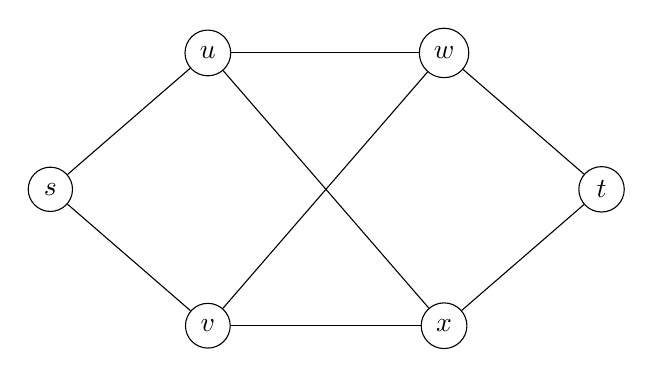
\begin{tikzpicture}[
		wide/.style={line width=4pt},
		every node/.style={circle,draw,minimum size=16},
		scale=2]
		\node (s) at (-0.5,0)            {$s$};
		\node (u) at ($ (0,0) + ( 60:1)$) {$u$};
		\node (v) at ($ (0,0) + (-60:1)$) {$v$};
		\node (w) at ($ (u) + ( 1.5,0 )$) {$w$};
		\node (x) at ($ (v) + ( 1.5,0 )$) {$x$};
		\node (t) at ($ (w) + (-60:1) + (0.5,0)$) {$t$};
		\draw (s) -- (u);
		\draw (u) -- (w);
		\draw (w) -- (t);

% Replace the line \draw (w) -- (t); with the line below (after deleting the % symbol to uncomment) in order to draw a thicker edge.
%		\draw[line width=3pt] (w) -- (t);


		\draw (s) -- (v);
		\draw (v) -- (x);
		\draw (x) -- (t);
		\draw (u) -- (x);    
		\draw (v) -- (w);
		
\end{tikzpicture}
\end{center}

\item Let the root be $s$ and the single source shortest path tree, $T$ is depicted below. The edges $E_{T}$ are highlighted in dark green \\
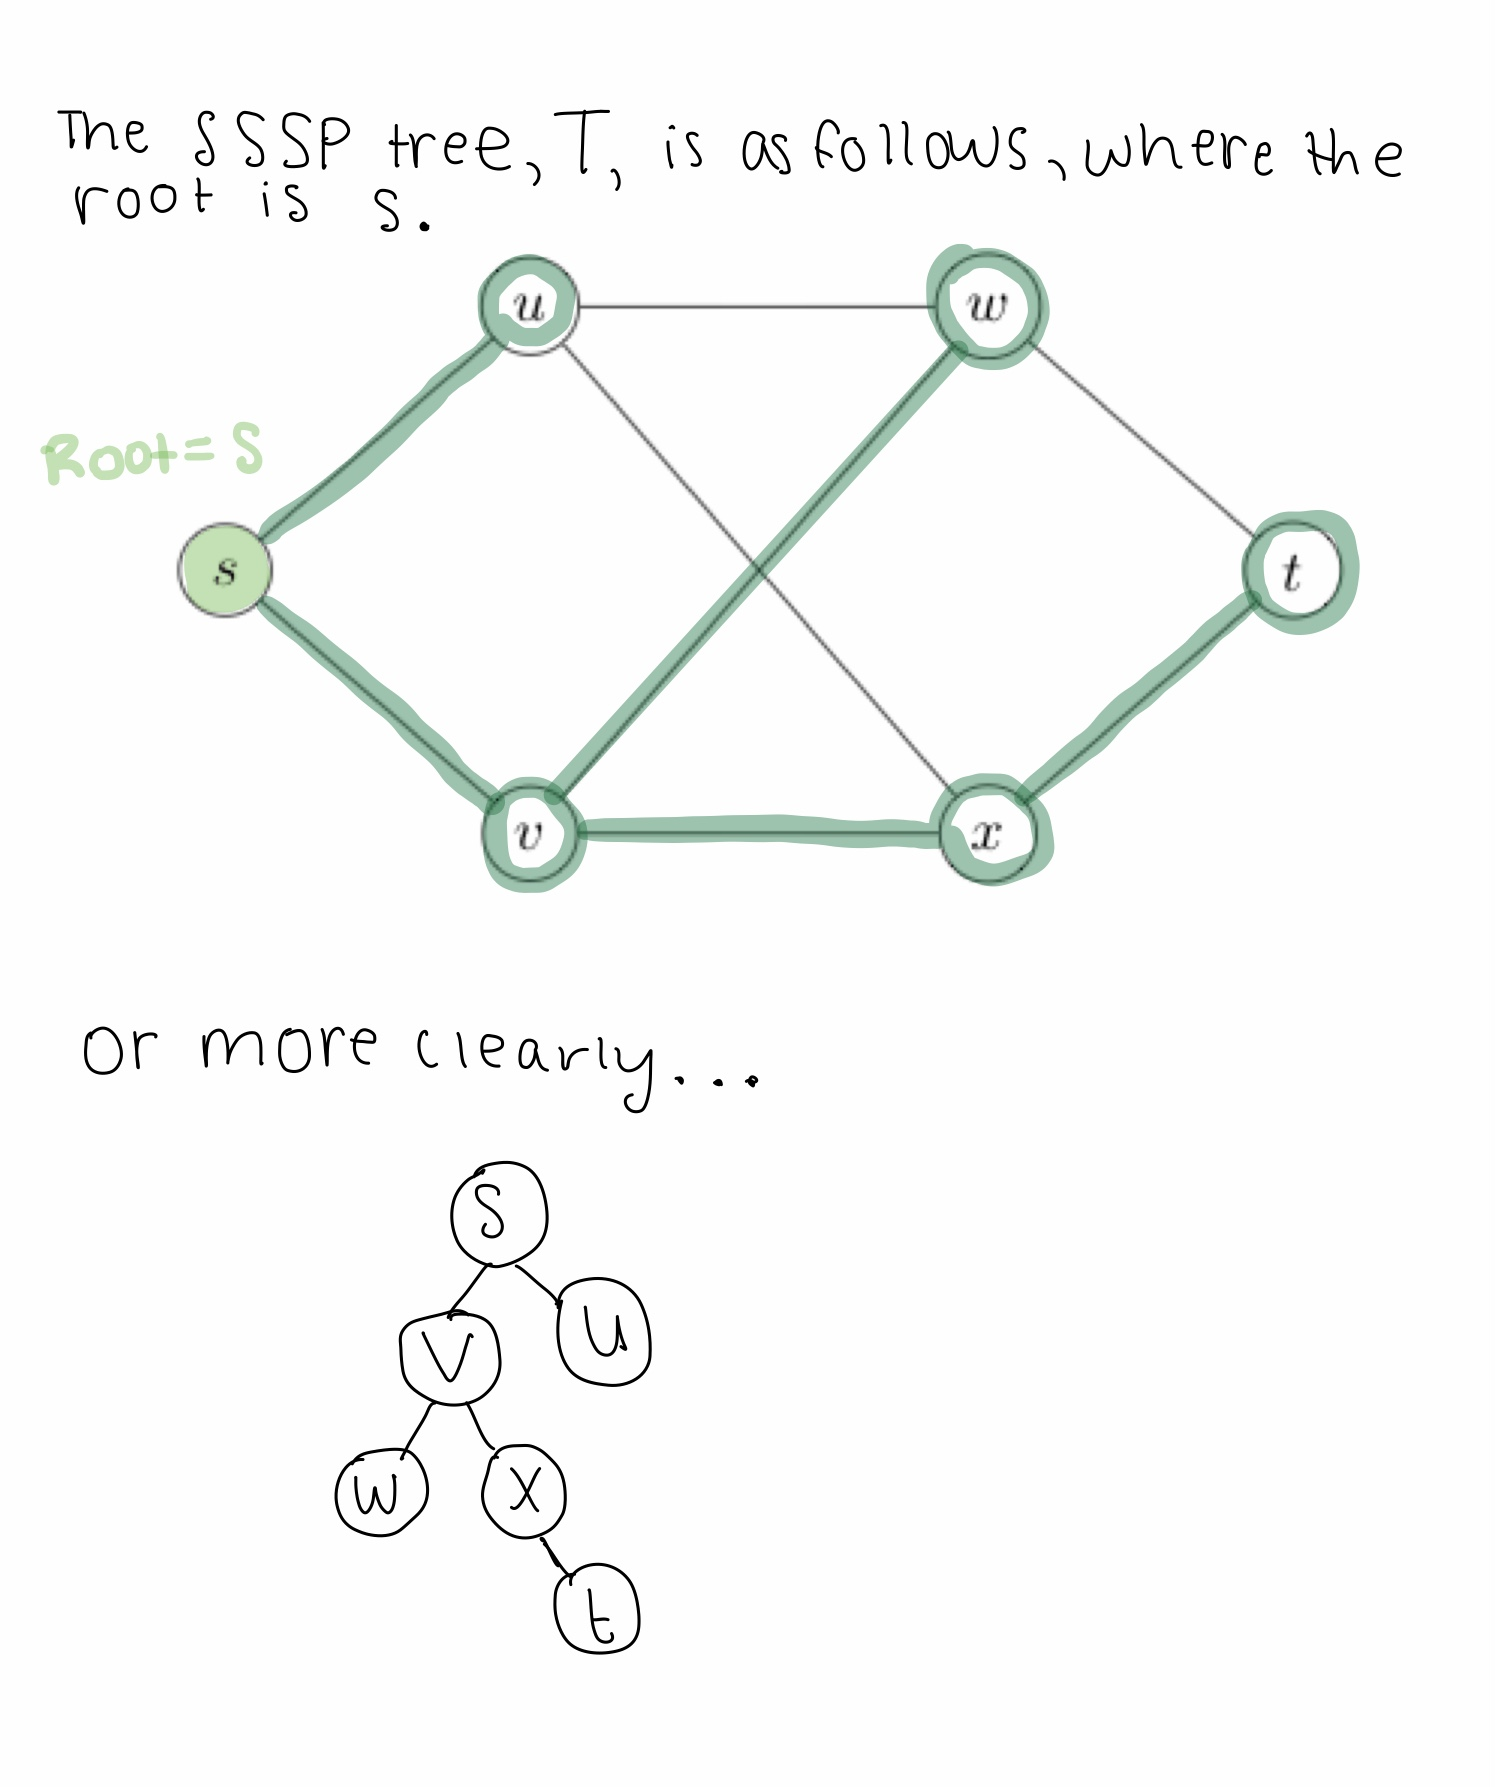
\includegraphics[width=0.5\textwidth]{hw2problem3} \\

\item A traditional DFS algorithm will never produce $T$ for any ordering of the vertices due to the way in which DFS traverses a graph. DFS uses a LIFO queue so it starts from a starting node, $s$, and recursively traverses the unvisited neighbors of $s$. This looks like: start at $s$, arbitrarily choose a neighbor to visit, call it $m$, then choose an arbitrary neighbor of $m$, say $n$ to visit, and repeats until it cannot find any more unvisited neighbors. At that point, backtrack until finding another unvisited neighbor. The result of this are long stringy trees. 


\end{enumerate}
\end{proof}








\newpage
\subsection{Problem \ref{DFS4}}
\begin{required} \label{DFS4}
	Give an example of a simple, undirected, weighted graph such that a breadth-first traversal outputs a search-tree that is not a single source shortest path tree. (That is, BFS is not sufficiently powerful to solve the shortest-path problem on weighted graphs. This motivates Dijkstra's algorithm.) 
	Your answer must
	\begin{enumerate}[label=(\alph*)]
		\item Draw the graph $G = (V,E, w)$ by specifying $V$ and $E$, clearly labeling the edge weights.  [\textbf{Note:} We have provided TikZ code below if you wish to use \LaTeX \ to draw the graph. Alternatively, you may hand-draw $G$ and embed it as an image below, provided that (i) your drawing is legible and (ii) we do not have to rotate our screens to grade your work.]
		\item Specify a spanning tree $T(V, E_{T})$ that is returned by BFS, but is not a single-source shortest path tree. [\textbf{Note:} You may again hand-draw this tree. If you wish, you may clearly mark the edges of $T$ on your drawing of $G$. Please make it easy on the graders to identify the edges of $T$.] 

		\item Specify a valid single-source shortest path tree $T^{\prime} = (V,E_{T^{\prime}})$.  [\textbf{Note:} You may again hand-draw this tree. If you wish, you may clearly mark the edges of $T$ on your drawing of $G$. Please make it easy on the graders to identify the edges of $T$.] 

		\item Include a clear explanation of why the search-tree output by breadth-first search is not a valid single-source shortest path tree of $G$.
	\end{enumerate}
\end{required}


\begin{proof}[Answer]
%Your answer here.
	\begin{enumerate}[label=(\alph*)]
		\item The graph $G = (V,E, w)$ is depicted below\\
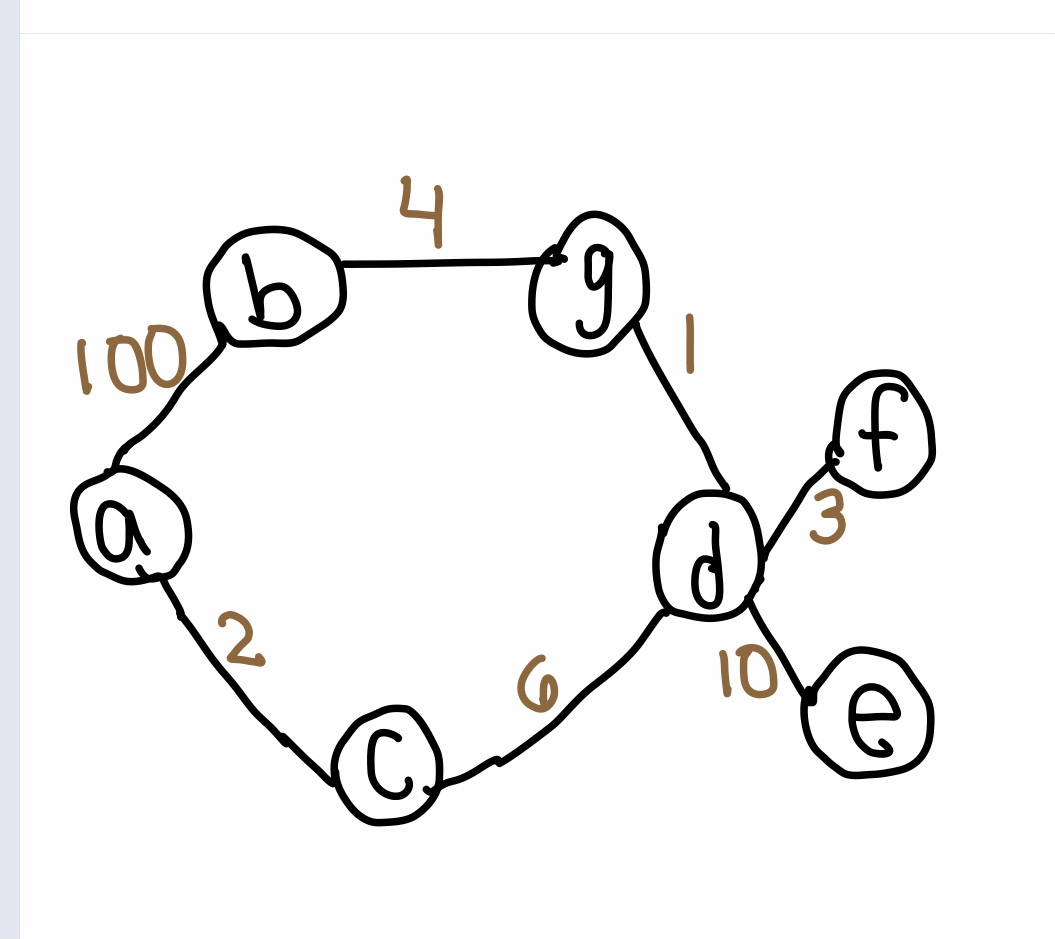
\includegraphics[width=0.5\textwidth]{hw2problem4a} 


		\item A spanning tree $T(V, E_{T})$ that is returned by BFS, but is not a single-source shortest path tree is depicted below. Let vertex $A$ be the starting vertex. \\
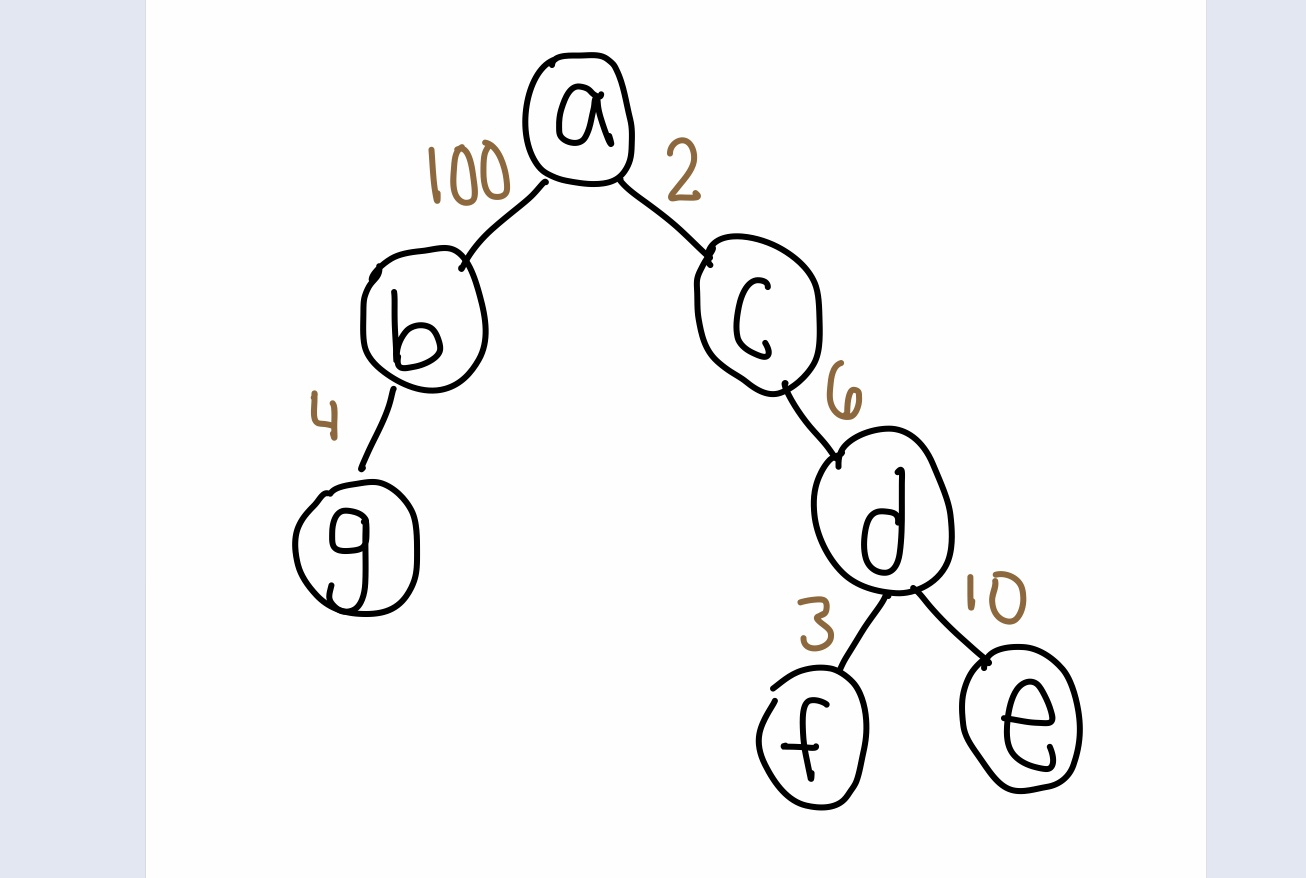
\includegraphics[width=0.5\textwidth]{hw2problem4b} 

		\item A valid single-source shortest path tree $T^{\prime} = (V,E_{T^{\prime}})$ is depicted below. Let vertex $A$ be the starting vertex. \\
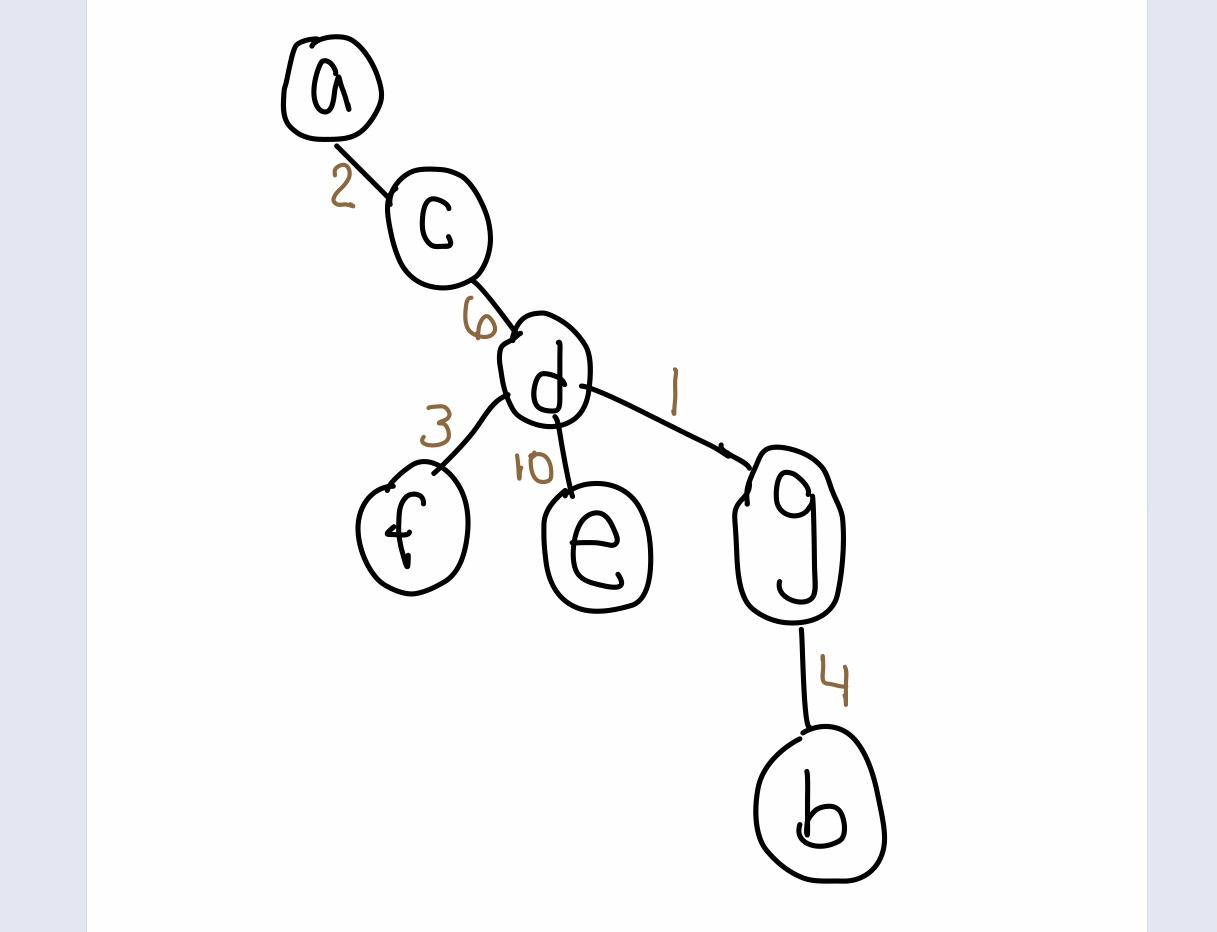
\includegraphics[width=0.5\textwidth]{hw2problem4c} 

		\item The search-tree output by breadth-first search is not a valid single-source shortest path tree of $G$ because BFS only produces valid SSSP trees for UNWEIGHTED graphs, or if all of the weights of edges are the same. This is because BFS counts the number of edges, rather than the weight of the edges. BFS finds all the vertices that are 1 edge away from the starting vertex, then 2 edges away, etc until it has visited all vertices. Hence, BFS minimizes the number of edges that are traversed, rather than considering the weight of the edges. \\
So, in the graph above, where $A$ is the starting vertex, BFS finds the following paths: \\
\begin{itemize}
\item $A$ to $B$: $A-B$ with a weight of 100 \\
\item $A$ to $G$: $A-B-G$ with a weight of 104 \\
\item $A$ to $C$: $A-C$ with a weight of 2 \\
\item $A$ to $D$: $A-C-D$ with a weight of 8 \\
\item $A$ to $F$: $A-C-D-F$ with a weight of 11 \\
\item $A$ to $E$: $A-C-D-E$ with a weight of 18 
\end{itemize}
However, the correct shortest paths (which Dijkstra's correctly finds) are:
\begin{itemize}
\item $A$ to $B$: $A-C-D-G-B$ with a weight of 13\\
\item $A$ to $G$: $A-C-D-G$ with a weight of 9 \\
\item $A$ to $C$: $A-C$ with a weight of 2 \\
\item $A$ to $D$: $A-C-D$ with a weight of 8 \\
\item $A$ to $F$: $A-C-D-F$ with a weight of 11 \\
\item $A$ to $E$: $A-C-D-E$ with a weight of 18 
\end{itemize}

	\end{enumerate}


\end{proof}


%%%%%%%%%%%%%%%%%%%%%%%%%%%%%%%%%%%%%%%%%%%%%%%%%%


\newpage
\section{Standard 6- Dijkstra's Algorithm}

\subsection{Problem \ref{Dijkstra0}}
\begin{required} \label{Dijkstra0}
Consider the weighted graph $G(V, E, w)$ pictured below. Work through Dijkstra's algorithm on the following graph, using the source vertex $E$. 
\begin{itemize}
\item Clearly include the contents of the priority queue, as well as the distance from $E$ to each vertex at each iteration.
\item If you use a table to store the distances, clearly label the keys according to the vertex names rather than numeric indices (i.e., \texttt{dist[`B']} is more descriptive than \texttt{dist[`1']}).
\item You do \textbf{not} need to draw the graph at each iteration, though you are welcome to do so. [This may be helpful scratch work, which you do not need to include.]
\end{itemize}


\begin{center}
\begin {tikzpicture}[-latex, auto, node distance =2 cm and 3cm, semithick]
\tikzstyle{blue}=[circle ,top color =white , bottom color = processblue!20 ,draw,processblue , text=blue , minimum width =1 cm];
\tikzstyle{red}=[circle ,top color =white , bottom color = processred!20 ,draw, processred , text=blue , minimum width =1 cm];
\tikzstyle{green}=[circle ,top color =white , bottom color = processgreen!20 ,draw, processgreen , text=blue , minimum width =1 cm];

	\node[blue] (A) {$A$};
	\node[blue] (C) [below right = of A] {$C$};
	\node[blue] (B) [below right = of C] {$B$};
	\node[blue] (E) [below left = of A] {$E$};
	\node[blue] (D) [below left = of E] {$D$};
	\node[blue] (H) [below right = of D] {$H$};
	\node[blue] (F) [right = of H] {$F$};

	\path (A) edge node[above] {$4$} (C);
	\path (E) edge node[left] {$9$} (A);

	\path (C) edge node[above] {$3$} (B);
	\path (B) edge node[below] {$6$} (F);

	\path (E) edge node[above] {$10$} (C);
	\path (C) edge node[above] {$2$} (F);

	\path (D) edge node[above] {$4$} (H);

	\path (E) edge node[above] {$20$} (F);
	\path (E) edge node[right] {$9$} (D);
	\end{tikzpicture}  
\end{center}

\end{required}

\begin{proof}[Answer]
%Your answer here

We invoke $Dijkstra(G, E)$, where $E$ is the starting vertex \\

\begin{enumerate}
\item For all vertices except $E$, set the distance to $\infty$. Set $E.dist= 0$ and push $E$ on the priority queue so that $Q= [(E,0)]$
\item Poll E. Set $E$.processed= true. The unprocessed neighbors of $E$ are $A, C, F, D$. 
	\begin{itemize}
	\item $w({E,A})= 9 < \infty$ so $A.dist=9$ and $A.predecessor= E$
	\item $w({E,C})= 10 < \infty$ so $C.dist=10$ and $C.predecessor= E$
	\item $w({E,F})= 20 < \infty$ so $F.dist=20$ and $F.predecessor= E$
	\item $w({E,D})= 9 < \infty$ so $D.dist=9$ and $D.predecessor= E$  \\
	Push $A, C, F, D$ to the priority queue so $Q= [(A,9), (D,9), (C,10), (F,20)]$
	\end{itemize}
\item Poll A from the priority queue and set A.processed=true. The unprocessed neighbor of $A$ is $C$.
	\begin{itemize}
	\item $dist(E,A) + w({A,C})= 9+4 > 10$ so we make no further changes to $C$\\
	Now the priority $Q= [(D,9), (C,10), (F,20)]$
	\end{itemize}
\item Poll D from the priority queue and set D.processed=true. The unprocessed neighbor of $D$ is $H$.
	\begin{itemize}
	\item $dist(E,D) + w({D,H})= 9+4 < \infty $ so $H.dist=13$ and $H.predecessor= D$\\
	Push $H$ to the priority queue so $Q= [(C,10), (H,13), (F,20)]$
	\end{itemize}
\item Poll C from the priority queue and set C.processed=true. The unprocessed neighbors of $C$ are $B$ and $F$.
	\begin{itemize}
	\item $dist(E,C) + w({C,B})= 10+3 < \infty $ so $B.dist=13$ and $B.predecessor= C$
	\item $dist(E,C) + w({C,F})= 10+2 < 20 $ so $F.dist=12$ and $F.predecessor= C$\\
	Push $B$ to the priority queue and reorder so now $Q= [(F,12), (H,13), (B,13)]$
	\end{itemize}
\item Poll F from the priority queue and set F.processed=true. The unprocessed neighbor of $F$ is $B$.
	\begin{itemize}
	\item $dist(E,F) + w({F,B})= 12+6 > 13 $ so we make no further changes to $B$ \\
	Now $Q= [(H,13), (B,13)]$
	\end{itemize}
\item Poll $H$ from the priority queue and set H.processed=true. There are no unprocessed neighbors of $H$ so $Q= [(B,13)]$
\item Poll $B$ from the priority queue and set B.processed=true. As there are no unprocessed neighbors of $B$ and the queue is empty, so the algorithm terminates\\
\end{enumerate}
 Dijkstra's found the shortest paths from $E$ to each vertex.
		\begin{itemize}
		\item $E$ to $A$: $E-A$ which has a weight 9. 
		\item $E$ to $D$: $E-D$ which has a weight 9. 
		\item $E$ to $C$: $E-C$ which has a weight 10. 
		\item $E$ to $F$: $E-C-F$ which has a weight 12. 
		\item $E$ to $B$: $E-C-B$ which has a weight 13. 
		\item $E$ to $H$: $E-D-H$ which has a weight 13. 

		\end{itemize}

\end{proof}





\newpage
\subsection{Problem \ref{Dijkstra2}} 
\begin{required} \label{Dijkstra2}
You have three batteries, with capacities of 40, 25, and 16 Ah (Amp-hours), respectively. The 25 and 16-Ah batteries are fully charged (containing 25 Ah and 16 Ah, respectively), while the 40-Ah battery is empty, with 0 Ah. You have a battery transfer device which has a ``source'' battery position and a ``target'' battery position. When you place two batteries in the device, it instantaneously transfers as many Ah from the source battery to the target battery as possible. Thus, this device stops the transfer either when the source battery has no Ah remaining or when the destination battery is fully charged (whichever comes first).  \\

\noindent But battery transfers aren't free! The battery device is also hooked up to your phone by bluetooth, and automatically charges you a number of dollars equal to however many Ah it just transfered.  \\
	
\noindent The goal in this problem is to determine whether there exists a sequence of transfers that leaves exactly 10 Ah either in the 25-Ah battery or the 16-Ah battery, and if so, how little money you can spend to get this result. \\

\noindent Do the following.
\begin{enumerate}[label=(\alph*)]
\subsubsection{Problem 6\ref{Dijkstra2a}}
\item \label{Dijkstra2a} Rephrase this is as a graph problem. Give a precise definition of how to model this problem as a graph, and state the specific question about this graph that must be answered. [\textbf{Note:} While you are welcome to draw the graph, it is enough to provide 1-2 sentences clearly describing what the vertices are and when two vertices are adjacent. If the graph is weighted, clearly specify what the edge weights are.]

\begin{proof}[Answer]
%Your answer goes here.
Given a graph $G(V, E, W)$ where each vertex $V$ is a tuple holding the charge of the batteries such that each $V= [$Charge of $40Ah$, Charge of $25Ah$, Charge of $16Ah]$. When two vertices are adjacent, this represents a batter transfer so each edge, $E$ represents 1 battery transfer such that the weight of the edge indicates the number of Ah transferred. So each edge weight = amount of Ah transferred. \\
The goal is to find the shortest weight path from the start vertex $[0,25,16]$ to a vertex where the 2nd or the 3rd element is $10$. That is, find the shortest path from $[0,25,16]$ to  $[xx, 10, xx]$ or $[xx,xx,10]$, where $xx$ represents some arbitrary number. \\

A representation of the graph is seen below\\
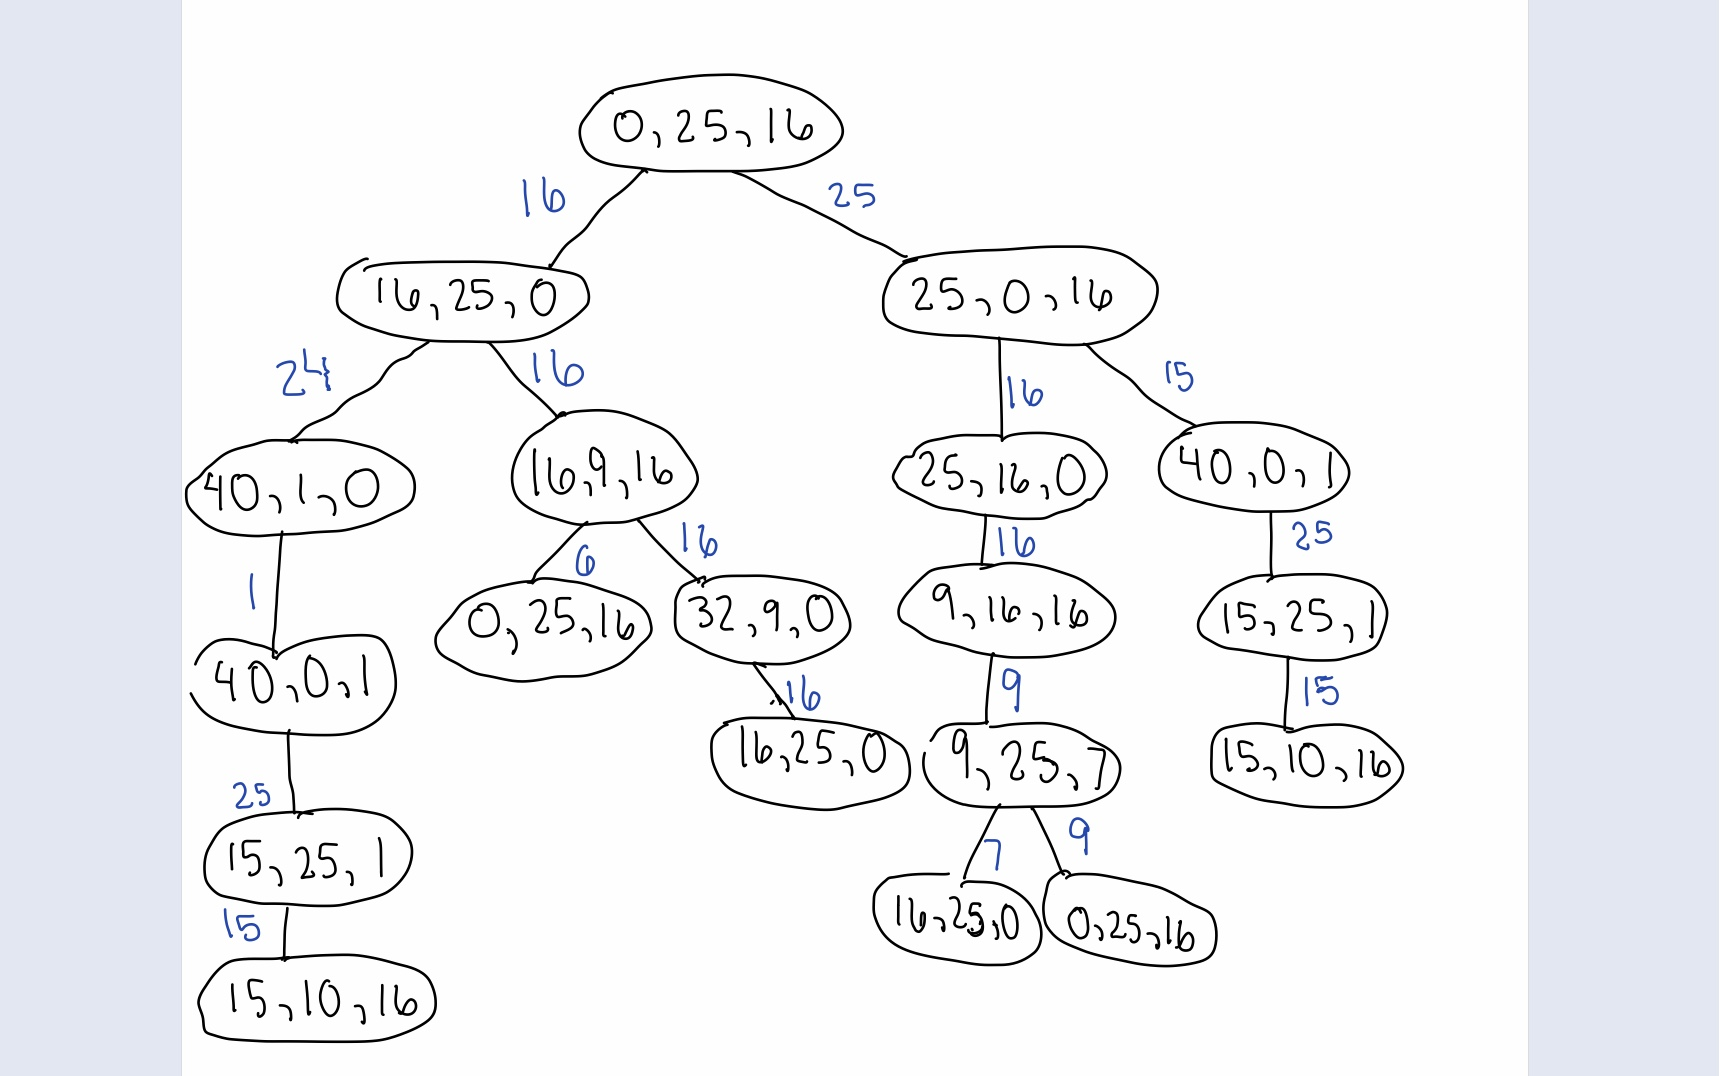
\includegraphics[width=0.5\textwidth]{hw2problem6a} \\


\end{proof}

\newpage
\subsubsection{Problem 6\ref{Dijkstra2b}}
\item \label{Dijkstra2b} Clearly describe an algorithm to solve this problem. If you use an algorithm covered in class, it is enough to state that. If you modify an algorithm from class, clearly outline any modifications. Make sure to explicitly specify any parameters that need to be passed to the initial function call.

\begin{proof}[Answer]
%Your answer goes here
Dijkstra's algorithm can be used to solve this problem. Call Dijkstra's from the starting vertex $[0,25,16]$. After Dijkstra's terminates, we will have the shortest path to all vertices. But since there will be multiple vertices with the form $[xx, 10, xx]$ or $[xx,xx,10]$, we will compare the weight of each of them and choose the lowest one.
\end{proof}



\newpage
\subsubsection{Problem 6\ref{Dijkstra2c}}
\item \label{Dijkstra2c} Apply that algorithm to the question. Report and justify your answer. Here, justification includes the sequences of vertices visited and the total cost. 

\begin{proof}[Answer]
%Your answer goes here. 
Using the following graph, where I have labeled the vertices for simplicity, we invoke $Dijkstra(G, A)$, where $A$ is the starting vertex, $[0,25,16]$ \\
 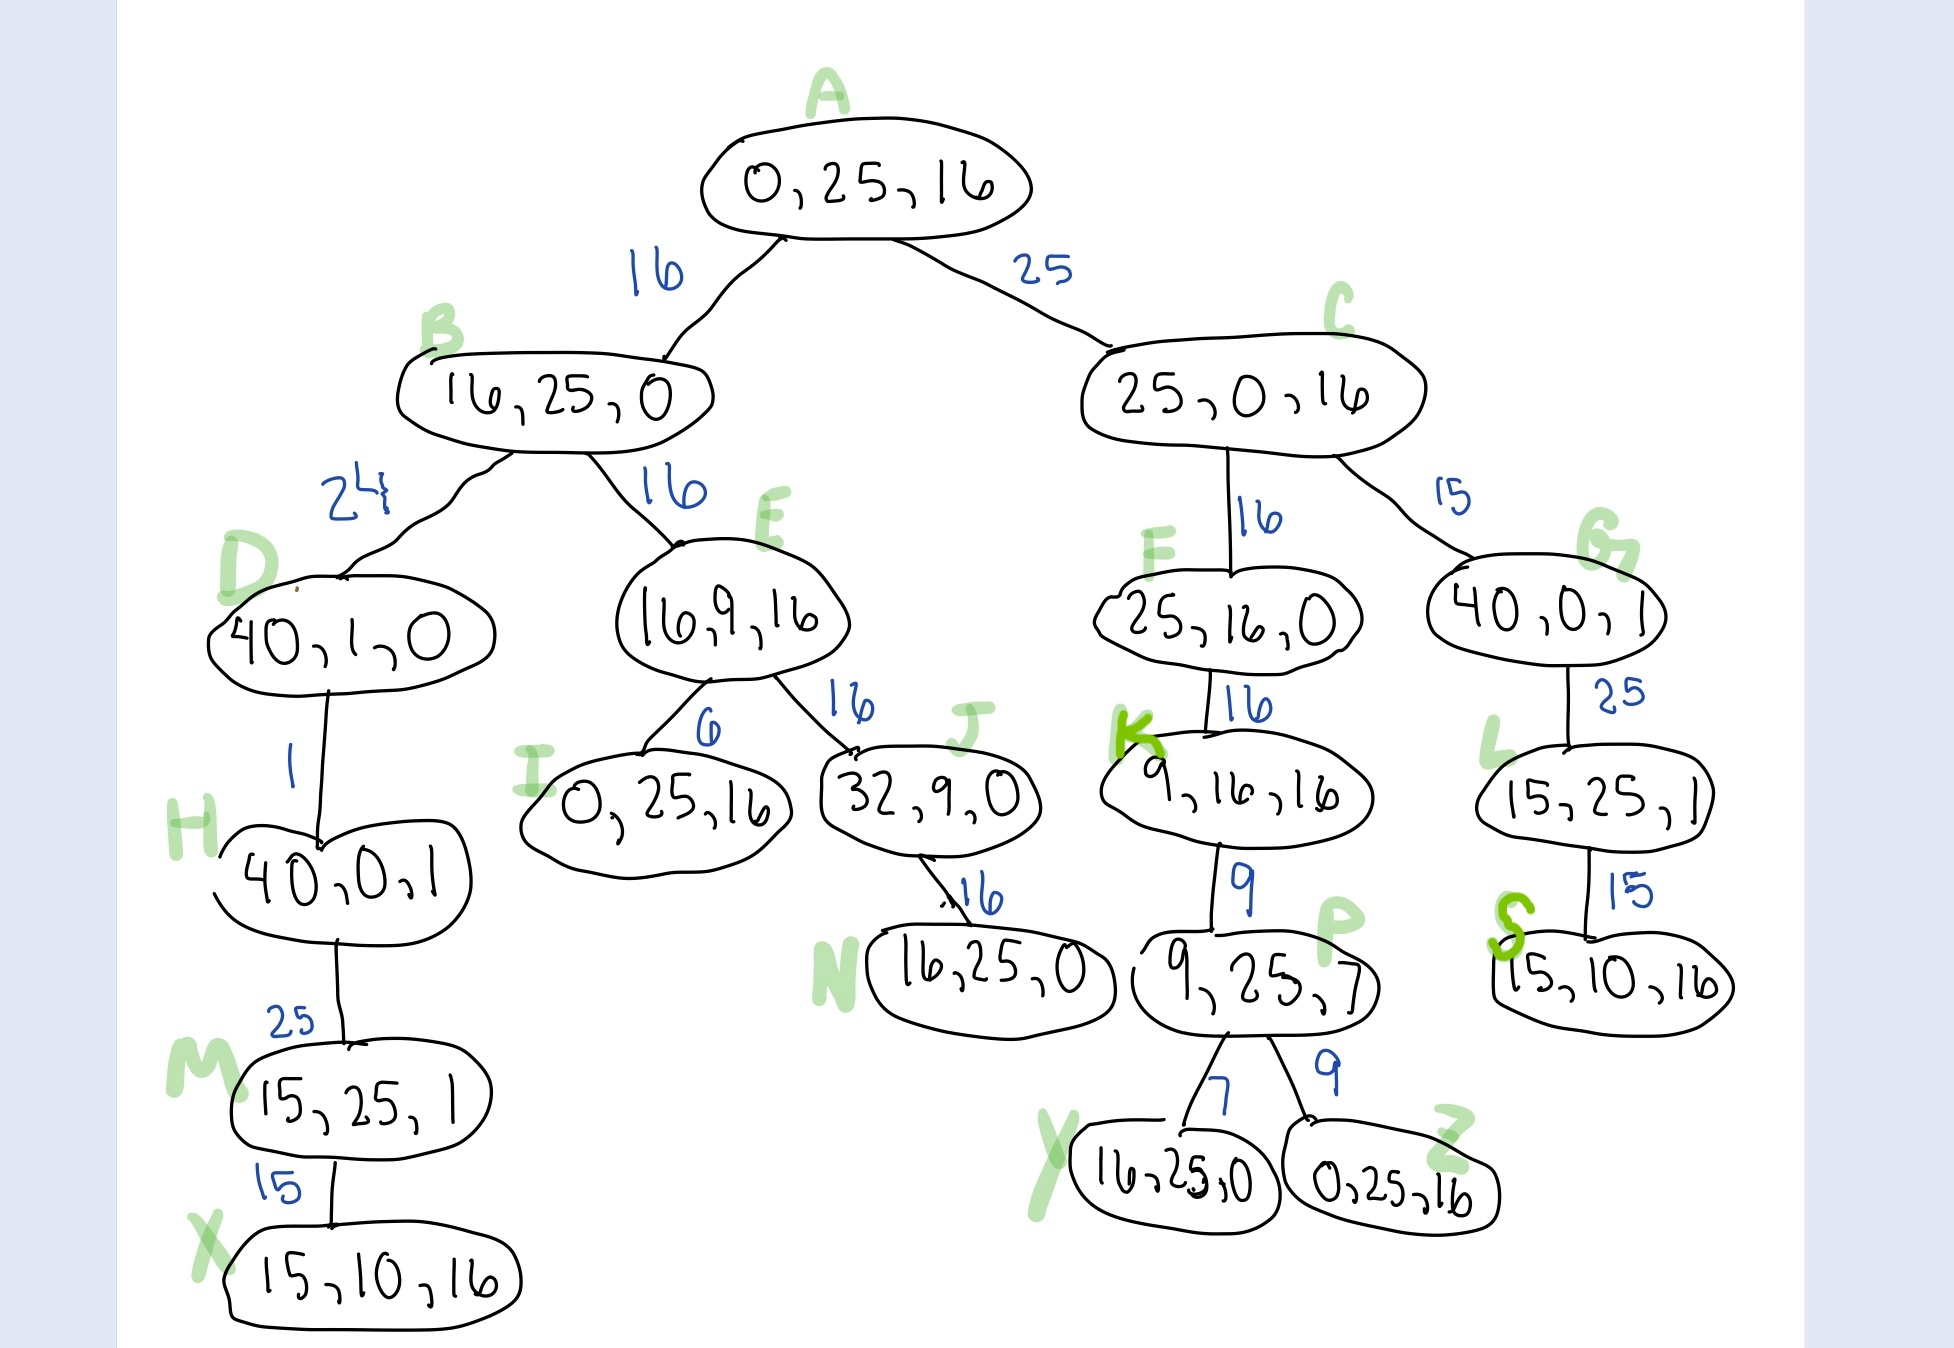
\includegraphics[width=0.8\textwidth]{hw2problem6c} \\

\begin{enumerate}[label=\arabic*)]
\item For all vertices except $A$, set the distance to $\infty$. Set $A.dist= 0$ and push $A$ on the priority queue so that $Q= [(A,0)]$
\item Poll A. Set $A$.processed= true. The unprocessed neighbors of $A$ are $B, C$. 
	\begin{itemize}
	\item $w({A,B})= 16 < \infty$ so $B.dist=16$ and $B.predecessor= A$
	\item $w({A,C})= 25 < \infty$ so $C.dist=10$ and $C.predecessor= A$
	Push $B, C$ to the priority queue so $Q= [(B,16), (C,25)]$
	\end{itemize}
\item Poll B from the priority queue and set B.processed=true. The unprocessed neighbors of $B$ are $D, E$.
	\begin{itemize}
	\item $dist(A,B) + w({B,D})= 16+24 < \infty$  so $D.dist=40$ and $D.predecessor= B$\\
	\item $dist(A,B) + w({B,E})= 16+16 < \infty$  so $E.dist=32$ and $E.predecessor= B$\\
	Now the priority $Q= [(C,25), (D,40), (E,32)]$
	\end{itemize}
\item Poll C from the priority queue and set C.processed=true. The unprocessed neighbors of $C$ are $F, G$.
	\begin{itemize}
	\item $dist(A,C) + w({C,F})= 25+16 < \infty $ so $F.dist=41$ and $F.predecessor= C$\\
	\item $dist(A,C) + w({C,G})= 25+15 < \infty $ so $G.dist=40$ and $G.predecessor= C$\\
	Push $F, G$ to the priority queue so $Q= [(D,40), (E,32), (G,40), (F,41)]$
	\end{itemize}
\item Poll D, mark it as processed, add H to the priority queue. $Q= [(E,32), (G,40), (F,41), (H,41)]$
\item Poll E, mark it as processed add I and J to the priority queue. $Q= [(I,38), (G,40), (F,41), (H,41), (J,48)]$
\item Poll I, mark it as processed, since it has no neighbors, nothing is added. $Q= [(G,40), (F,41), (H,41), (J,48)]$
\item Poll G, mark it as processed, add L to the priority queue. $Q= [(F,41), (H,41), (J,48), (L,65)]$
\item Poll F, mark it as processed, add K to the priority queue. $Q= [(H,41), (J,48), (K,57), (L,65)]$
\item Poll H, mark it as processed, add M to the priority queue. $Q= [(J,48), (K,57), (L,65), (M,66)]$
\item Poll J, mark it as processed, add N to the priority queue. $Q= [(K,57), (N,64),(L,65), (M,66)]$
\item Poll K, mark it as processed, add P to the priority queue. $Q= [(N,64),(L,65), (M,66), (P,66)]$
\item Poll N, mark it as processed, since it has no neighbors, nothing is added. $Q= [(L,65), (M,66), (P,66)]$
\item Poll L, mark it as processed, add S to the priority queue. $Q= [(M,66), (P,66),(S,80)]$
\item Poll M, mark it as processed, add X to the priority queue. $Q= [(P,66),(S,80),(X,81)]$
\item Poll P, mark it as processed, add Y and Z to the priority queue. $Q= [(Y,73),(Z,75),(S,80),(X,81)]$
\item Poll Y, mark it as processed, since it has no neighbors, nothing is added. $Q= [(Z,75),(S,80),(X,81)]$
\item Poll Z, mark it as processed, since it has no neighbors, nothing is added. $Q= [(S,80),(X,81)]$
\item Poll S, mark it as processed, since it has no neighbors, nothing is added. $Q= [(X,81)]$
\item Poll X, mark it as processed, since it has no neighbors, nothing is added. Now the queue is empty and the algorithm terminates.
\end{enumerate}
 Dijkstra's found the shortest paths from $A$, which is $[0,25,16]$ to each vertex in the graph. Since we are only interested in the vertices that are  $[xx, 10, xx]$ or $[xx,xx,10]$, we will only examine those. The vertices of that form correspond to $X$ and $S$, which are $[15,10,16]$ and $[15, 10, 16]$.
		\begin{itemize}
		\item $A$ to $X$, which is $[0, 25, 16]$ to $[15,10,16]$: has a weight 81 and the path is \\ $[0, 25, 16]-[15, 25, 0]-[40, 1, 0]-[40, 0, 1]-[15, 25, 1]-[15, 10, 16]$. 
		\item $A$ to $S$, which is $[0, 25, 16]$ to $[15,10,16]$: has a weight 80 and the path is \\ $[0, 25, 16]-[25, 0, 16]-[40, 0, 1]-[15, 25, 1]-[15, 10, 16]$. 
		\end{itemize}
Since $80 < 81$, the cheapest sequence of transfers to result with 10Ah in the 25Ah or 16Ah battery is \\ $[0, 25, 16]-[25, 0, 16]-[40, 0, 1]-[15, 25, 1]-[15, 10, 16]$. Thus 80 is the cheapest way to achieve the goal.
\end{proof}
\end{enumerate}
\end{required}



\end{document} % NOTHING AFTER THIS LINE IS PART OF THE DOCUMENT



